\begin{figure}[h]
  \begin{center}
    \begin{adjustbox}{width=0.7\columnwidth}
        \tikzset{every picture/.style={line width=0.75pt}} %set default line width to 0.75pt        
            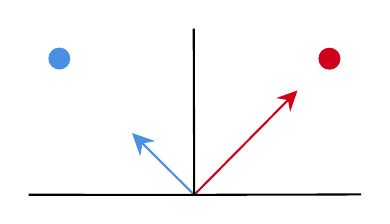
\begin{tikzpicture}[x=0.75pt,y=0.75pt,yscale=-1,xscale=1]
            %uncomment if require: \path (0,300); %set diagram left start at 0, and has height of 300
            
            %Straight Lines [id:da17586827840068286] 
            \draw [color={rgb, 255:red, 208; green, 2; blue, 27 }  ,draw opacity=1 ]   (190.24,200.32) -- (237.89,152.16) ;
            \draw [shift={(240,150.03)}, rotate = 494.69] [fill={rgb, 255:red, 208; green, 2; blue, 27 }  ,fill opacity=1 ][line width=0.08]  [draw opacity=0] (9.82,-4.72) -- (0,0) -- (9.82,4.72) -- (6.52,0) -- cycle    ;
            %Straight Lines [id:da23704064540856618] 
            \draw [color={rgb, 255:red, 74; green, 144; blue, 226 }  ,draw opacity=1 ]   (190.24,200.32) -- (162.38,172.64) ;
            \draw [shift={(160.25,170.53)}, rotate = 404.81] [fill={rgb, 255:red, 74; green, 144; blue, 226 }  ,fill opacity=1 ][line width=0.08]  [draw opacity=0] (10.72,-5.15) -- (0,0) -- (10.72,5.15) -- (7.12,0) -- cycle    ;
            %Shape: Circle [id:dp3839733612485111] 
            \draw  [color={rgb, 255:red, 208; green, 2; blue, 27 }  ,draw opacity=1 ][fill={rgb, 255:red, 208; green, 2; blue, 27 }  ,fill opacity=1 ] (250.58,134.73) .. controls (250.58,132.08) and (252.73,129.93) .. (255.38,129.93) .. controls (258.03,129.93) and (260.18,132.08) .. (260.18,134.73) .. controls (260.18,137.38) and (258.03,139.53) .. (255.38,139.53) .. controls (252.73,139.53) and (250.58,137.38) .. (250.58,134.73) -- cycle ;
            %Shape: Circle [id:dp009447430116501954] 
            \draw  [color={rgb, 255:red, 74; green, 144; blue, 226 }  ,draw opacity=1 ][fill={rgb, 255:red, 74; green, 144; blue, 226 }  ,fill opacity=1 ] (120.47,134.66) .. controls (120.47,132.02) and (122.61,129.88) .. (125.25,129.88) .. controls (127.89,129.88) and (130.03,132.02) .. (130.03,134.66) .. controls (130.03,137.29) and (127.89,139.43) .. (125.25,139.43) .. controls (122.61,139.43) and (120.47,137.29) .. (120.47,134.66) -- cycle ;
            %Straight Lines [id:da5714219654763008] 
            \draw    (190,120.28) -- (190.24,200.32) ;
            %Straight Lines [id:da22247567054966455] 
            \draw    (110.5,200.28) -- (190.24,200.32) ;
            %Straight Lines [id:da4124676757039665] 
            \draw    (270.64,200.12) -- (190.24,200.32) ;
            
            
            
            
            \end{tikzpicture}
    \end{adjustbox}
  \end{center}
\caption{\textbf{Motivation as a vector}. Blue and red dots represent two objects with different characteristics while the two arrows illustrate the hypothetical motivational propensity of an individual (or two individuals) towards them. The black segments delineate the space created by the combination of the objects' characteristics and the motivational propensity of the individuals. Here the red object has the potential to generate more behaviour than the blue object possibly as a result of its characteristics and those of the individual interacting with it.}
\label{fig: vect_mot}
\end{figure}